% 57-80(57쪽) — 구간 [α, β] 에서 평균값 정리를 묻는 문항의 y=f(x) 그래프. 스캔 화질이 낮아 TikZ 로 다시 그림.
% 원문에 있는 것만: x축 위 문자 α, β · 그 두 곳의 세로 안내 파선 · 라벨 O, x, y, y=f(x) · 구간 밖은 파선.
% 눈금 숫자는 원문에 없으므로 넣지 않는다(개수를 세는 문항이라 수치를 더하면 답이 드러난다).
% 곡선은 원문 모양 그대로 지나는 점들을 재서 smooth 로 잇는다(식이 주어진 그래프가 아니다).
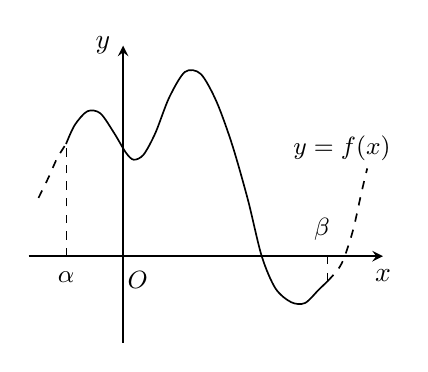
\begin{tikzpicture}[x=0.50cm, y=0.50cm, line width=0.5pt]
  \draw[->, >=stealth, line width=0.7pt] (-2.4,0) -- (6.6,0) node[below=1pt] {$x$};
  \draw[->, >=stealth, line width=0.7pt] (0,-2.2) -- (0,5.35) node[left=1pt] {$y$};
  \node[below=2pt, font=\small] at (0.37,0) {$\pt{O}$};
  % 구간 끝의 세로 안내 파선(원문: α 는 축 위로, β 는 축 아래로)
  \draw[dashed, line width=0.35pt] (-1.45,0) -- (-1.45,2.85);
  \draw[dashed, line width=0.35pt] (5.20,0) -- (5.20,-0.63);
  % 그래프 — 구간 [α, β] 밖은 원문처럼 파선
  \draw[dashed, line width=0.6pt, smooth] plot coordinates {(-2.15,1.48) (-1.88,2.03) (-1.68,2.48) (-1.45,2.85)};
  \draw[line width=0.6pt, smooth] plot coordinates
    {(-1.45,2.85) (-1.23,3.33) (-0.91,3.68) (-0.58,3.63) (-0.23,3.13) (0.07,2.63) (0.27,2.45)
     (0.52,2.58) (0.82,3.13) (1.17,4.03) (1.57,4.68) (1.97,4.63) (2.37,3.93) (2.77,2.83)
     (3.17,1.43) (3.52,0) (3.87,-0.82) (4.27,-1.17) (4.62,-1.19) (4.97,-0.85) (5.20,-0.63)};
  \draw[dashed, line width=0.6pt, smooth] plot coordinates {(5.20,-0.63) (5.47,-0.32) (5.63,0) (5.85,0.70) (6.05,1.60) (6.20,2.23)};
  \node[below=2pt, font=\small] at (-1.45,0) {$\alpha$};
  \node[above=1pt, font=\small] at (5.05,0.08) {$\beta$};
  \node[right=1pt, font=\small] at (4.0,2.75) {$y=f(x)$};
\end{tikzpicture}
